\documentclass[12pt, a4paper]{article}
% Suppress reference warnings
\usepackage{silence}
\WarningFilter*{}{Label}
\WarningFilter{vntex}{No input encoding}

\usepackage[utf8]{inputenc}
\usepackage{vntex}
\usepackage[dvipsnames]{xcolor}
%\usepackage[english,vietnam]{babel}
%\usepackage[utf8]{inputenc}

%\usepackage[utf8]{inputenc}
%\usepackage[francais]{babel}
\usepackage{a4wide,amssymb,epsfig,latexsym,array,hhline,fancyhdr}
\usepackage[normalem]{ulem}
%\usepackage{soul}
\usepackage{caption}
\usepackage{float}
\renewcommand{\figurename}{}
\usepackage{wasysym}
\usepackage{enumitem}
\usepackage[makeroom]{cancel}
\let\iint\relax
\let\iiint\relax
\usepackage{amsmath}
\usepackage{amsfonts}
\usepackage{amssymb}
\usepackage{amsthm}
\usepackage{multicol,longtable,amscd}
\usepackage{diagbox}%Make diagonal lines in tables
\usepackage{booktabs}
\usepackage{alltt}
\usepackage[framemethod=tikz]{mdframed}% For highlighting paragraph backgrounds
\usepackage{caption,subcaption}
\usepackage{listings}
\usepackage{color}
\usepackage[lined,boxed,commentsnumbered]{algorithm2e}
\usepackage{enumerate}
\usepackage{graphicx}
\usepackage{array}
\usepackage{tabularx, caption}
\usepackage{multirow}
\usepackage{multicol}
\usepackage{rotating}
\usepackage{graphics}
\usepackage{geometry}
\usepackage{setspace}
\usepackage{epsfig}
\usepackage{tikz}
\usepackage[colorlinks=true, linkcolor=blue, urlcolor=blue, unicode]{hyperref}
\usetikzlibrary{arrows,decorations.pathmorphing,backgrounds}

\hypersetup{urlcolor=blue,linkcolor=black,citecolor=black,colorlinks=true} 
%\usepackage{pstcol} % PSTricks with the standard color package

\newcolumntype{P}[1]{>{\centering\arraybackslash}p{#1}}

\newcolumntype{M}[1]{>{\centering\arraybackslash}m{#1}}

\newtheorem{theorem}{{\bf Định lý}}

\newtheorem{property}{{\bf Tính chất}}
\newtheorem{proposition}{{\bf Mệnh đề}}
\newtheorem{corollary}[proposition]{{\bf Hệ quả}}
\newtheorem{lemma}[proposition]{{\bf Bổ đề}}
\theoremstyle{definition}
\newtheorem{exer}{Bài toán}

\def\thesislayout{	% A4: 210 × 297
	\geometry{
		a4paper,
		total={160mm,240mm},  % fix over page
		left=30mm,
		top=30mm,
	}
}
\thesislayout%

%\usepackage{fancyhdr}
\setlength{\headheight}{40pt}
\pagestyle{fancy}
\fancyhead{} % clear all header fields
\fancyhead[L]{
 \begin{tabular}{rl}
    %\begin{picture}(25,15)(0,0)
    %\put(0,-8){\includegraphics[width=8mm, height=8mm]{hcmut.png}}
    %\put(0,-8){\epsfig{width=10mm,figure=hcmut.eps}}
   %\end{picture}&
	%\includegraphics[width=8mm, height=8mm]{hcmut.png} & %
	\begin{tabular}{l}
		\textbf{\bf \ttfamily Trường Đại Học Bách Khoa \textendash{} ĐHQG TP.HCM}\\
		\textbf{\bf \ttfamily Khoa Kỹ thuật và Khoa học Máy tính}
	\end{tabular} 	
 \end{tabular}
}
\fancyhead[R]{
	\begin{tabular}{l}
		\tiny \bf \\
		\tiny \bf 
	\end{tabular}  }
\fancyfoot{} % clear all footer fields
\fancyfoot[L]{\scriptsize \ttfamily Báo cáo bài tập lớn Vật lý Bán dẫn \textendash{} EE1007 \\ Niên khoá 2024 \textendash{} 2025}
\makeatletter
\fancyfoot[R]{\scriptsize \ttfamily Trang {\thepage}/\@ifundefined{r@LastPage}{?}{\pageref{LastPage}}}
\makeatother
\renewcommand{\headrulewidth}{0.3pt}
\renewcommand{\footrulewidth}{0.3pt}
%%%
\setcounter{secnumdepth}{4}
\setcounter{tocdepth}{3}
\makeatletter
\newcounter{subsubsubsection}[subsubsection]
\renewcommand\thesubsubsubsection{\thesubsubsection.\@alph\c@subsubsubsection}
\newcommand\subsubsubsection{\@startsection{subsubsubsection}{4}{\z@}%
                                     {-3.25ex\@plus -1ex \@minus -.2ex}%
                                     {1.5ex \@plus .2ex}%
                                     {\normalfont\normalsize\bfseries}}
\newcommand*\l@subsubsubsection{\@dottedtocline{3}{10.0em}{4.1em}}
\newcommand*{\subsubsubsectionmark}[1]{}
\makeatother

\everymath{\color{black}}%make in-line maths symbols blue to read/check easily

\sloppy
%\captionsetup[figure]{labelfont={small,bf},textfont={small,it},belowskip=-1pt,aboveskip=-9pt}
%space remove between caption, figure, and text
%\captionsetup[table]{labelfont={small,bf},textfont={small,it},belowskip=-1pt,aboveskip=7pt}
%space remove between caption, table, and text

%\floatplacement{figure}{H}%forced here float placement automatically for figures
%\floatplacement{table}{H}%forced here float placement automatically for table
%the following settings (11 lines) are to remove white space before or after the figures and tables
%\setcounter{topnumber}{2}
%\setcounter{bottomnumber}{2}
%\setcounter{totalnumber}{4}
%\renewcommand{\topfraction}{0.85}
%\renewcommand{\bottomfraction}{0.85}
%\renewcommand{\textfraction}{0.15}
%\renewcommand{\floatpagefraction}{0.8}
%\renewcommand{\textfraction}{0.1}
\setlength{\floatsep}{5pt plus 2pt minus 2pt}
\setlength{\textfloatsep}{5pt plus 2pt minus 2pt}
\setlength{\intextsep}{10pt plus 2pt minus 2pt}

\thesislayout%
% chktex 1 off
% chktex 8 off
\lstset{
language=C++,
    aboveskip=6mm,
    belowskip=-6mm,
    backgroundcolor=\color{white},   
    commentstyle=\color{codegreen},
    keywordstyle=\color{blue},
    numberstyle=\tiny\color{codegray},
    stringstyle=\color{codepurple},
    basicstyle=\ttfamily,
    breakatwhitespace=false,         
    breaklines=true,                 
    captionpos=b,                    
    keepspaces=true,                 
    numbers=left,                    
    numbersep=5pt,                  
    showspaces=false,                
    showstringspaces=false,
    showtabs=false,                  
    tabsize=2,
    frame=tb,
    framesep=8pt,
    rulecolor=\color{black},
    title=\lstname,
}

\usepackage{listings}

\usepackage{xcolor}

%New colors defined below
\definecolor{codegreen}{rgb}{0,0.6,0}
\definecolor{codegray}{rgb}{0.5,0.5,0.5}
\definecolor{codepurple}{rgb}{0.58,0,0.82}
\definecolor{backcolour}{rgb}{0.95,0.95,0.92}

%Code listing style named "mystyle"
\lstdefinestyle{mystyle}{
  backgroundcolor=\color{backcolour}, commentstyle=\color{codegreen},
  keywordstyle=\color{magenta},
  numberstyle=\tiny\color{codegray},
  stringstyle=\color{codepurple},
  basicstyle=\ttfamily\footnotesize,
  breakatwhitespace=false,         
  breaklines=true,                 
  captionpos=b,                    
  keepspaces=true,                 
  numbers=left,                    
  numbersep=5pt,                  
  showspaces=false,                
  showstringspaces=false,
  showtabs=false,                  
  tabsize=2
}

%"mystyle" code listing set
\lstset{style=mystyle}
\lstset{
        literate=%
% Vần a
	{á}{{\'a}}1
	{à}{{\`a}}1
	{ạ}{{\d a}}1
	{ả}{{\h a}}1
	{ã}{{\~ a}}1
	%
	{Á}{{\'A}}1
	{À}{{\`A}}1
	{Ạ}{{\d A}}1
	{Ả}{{\h A}}1
	{Ã}{{\~ A}}1
%
% Vần ă
	{ă}{{\u a}}1
	{ắ}{{\'\abreve }}1
	{ằ}{{\`\abreve }}1
	{ặ}{{\d \abreve }}1
	{ẳ}{{\h \abreve }}1
	{ẵ}{{\~\abreve }}1
	%
	{Ă}{{\u A}}1
	{Ắ}{{\'\ABREVE }}1
	{Ằ}{{\`\ABREVE }}1
	{Ặ}{{\d \ABREVE }}1
	{Ẳ}{{\h \ABREVE }}1
	{Ẵ}{{\~\ABREVE }}1
%
% Vần â
	{â}{{\^ a}}1
	{ấ}{{\'\acircumflex }}1
	{ầ}{{\`\acircumflex }}1
	{ậ}{{\d \acircumflex }}1
	{ẩ}{{\h \acircumflex }}1
	{ẫ}{{\~\acircumflex }}1
	 %
	{Â}{{\^ A}}1
	{Ấ}{{\'\ACIRCUMFLEX }}1
	{Ầ}{{\`\ACIRCUMFLEX }}1
	{Ậ}{{\d \ACIRCUMFLEX }}1
	{Ẩ}{{\h \ACIRCUMFLEX }}1
	{Ẫ}{{\~\ACIRCUMFLEX }}1
%
% Vần đ
	{đ}{{\dj }}1
	{Đ}{{\DJ }}1
%
% Vần e
	{é}{{\'e}}1
	{è}{{\`e}}1
	{ẹ}{{\d e}}1
	{ẻ}{{\h e}}1
	{ẽ}{{\~ e}}1
	%
	{É}{{\'E}}1
	{È}{{\`E}}1
	{Ẹ}{{\d E}}1
	{Ẻ}{{\h E}}1
	{Ẽ}{{\~ E}}1
%
% Vần ê
	{ê}{{\^e}}1
	{ế}{{\'\ecircumflex }}1
	{ề}{{\`\ecircumflex }}1
	{ệ}{{\d \ecircumflex }}1
	{ể}{{\h \ecircumflex }}1
	{ễ}{{\~\ecircumflex }}1
	%
	{Ê}{{\^E}}1
	{Ế}{{\'\ECIRCUMFLEX }}1
	{Ề}{{\`\ECIRCUMFLEX }}1
	{Ệ}{{\d \ECIRCUMFLEX }}1
	{Ể}{{\h \ECIRCUMFLEX }}1
	{Ễ}{{\~\ECIRCUMFLEX }}1
%
% Vần i
	{í}{{\'i}}1
	{ì}{{\`\i }}1
	{ị}{{\d i}}1
	{ỉ}{{\h i}}1
	{ĩ}{{\~\i }}1
	%
	{Í}{{\'I}}1
	{Ì}{{\`I}}1
	{Ị}{{\d I}}1
	{Ỉ}{{\h I}}1
	{Ĩ}{{\~I}}1
%
% Vần o
	{ó}{{\'o}}1
	{ò}{{\`o}}1
	{ọ}{{\d o}}1
	{ỏ}{{\h o}}1
	{õ}{{\~o}}1
	%
	{Ó}{{\'O}}1
	{Ò}{{\`O}}1
	{Ọ}{{\d O}}1
	{Ỏ}{{\h O}}1
	{Õ}{{\~O}}1
%
% Vần ô
	{ô}{{\^o}}1
	{ố}{{\'\ocircumflex }}1
	{ồ}{{\`\ocircumflex }}1
	{ộ}{{\d \ocircumflex }}1
	{ổ}{{\h \ocircumflex }}1
	{ỗ}{{\~\ocircumflex }}1
	%
	{Ô}{{\^O}}1
	{Ố}{{\'\OCIRCUMFLEX }}1
	{Ồ}{{\`\OCIRCUMFLEX }}1
	{Ộ}{{\d \OCIRCUMFLEX }}1
	{Ổ}{{\h \OCIRCUMFLEX }}1
	{Ỗ}{{\~\OCIRCUMFLEX }}1
%
% Vần ơ
	{ơ}{{\ohorn }}1
	{ớ}{{\'\ohorn }}1
	{ờ}{{\`\ohorn }}1
	{ợ}{{\d \ohorn }}1
	{ở}{{\h \ohorn }}1
	{ỡ}{{\~\ohorn }}1
	%
	{Ơ}{{\OHORN }}1
	{Ớ}{{\'\OHORN }}1
	{Ờ}{{\`\OHORN }}1
	{Ợ}{{\d \OHORN }}1
	{Ở}{{\h \OHORN }}1
	{Ỡ}{{\~\OHORN }}1
%
% Vần u
	{ú}{{\'u}}1
	{ù}{{\`u}}1
	{ụ}{{\d u}}1
	{ủ}{{\h u}}1
	{ũ}{{\~u}}1
	%
	{Ú}{{\'U}}1
	{Ù}{{\`U}}1
	{Ụ}{{\d U}}1
	{Ủ}{{\h U}}1
	{Ũ}{{\~U}}1
%
% Vần ư
	{ư}{{\uhorn }}1
	{ứ}{{\'\uhorn }}1
	{ừ}{{\`\uhorn }}1
	{ự}{{\d \uhorn }}1
	{ử}{{\h \uhorn }}1
	{ữ}{{\~\uhorn }}1
	%
	{Ư}{{\UHORN }}1
	{Ứ}{{\'\UHORN }}1
	{Ừ}{{\`\UHORN }}1
	{Ự}{{\d \UHORN }}1
	{Ử}{{\h \UHORN }}1
	{Ữ}{{\~\UHORN }}1
%
% Vần y
	{ý}{{\'y}}1
	{ỳ}{{\`y}}1
	{ỵ}{{\d y}}1
	{ỷ}{{\h y}}1
	{ỹ}{{\~y}}1
	%
	{Ý}{{\'Y}}1
	{Ỳ}{{\`Y}}1
	{Ỵ}{{\d Y}}1
	{Ỷ}{{\h Y}}1
	{Ỹ}{{\~Y}}1
}
% chktex 1 on
% chktex 8 on

\newmdenv[linecolor=black,skipabove=10pt,skipbelow=0pt,innertopmargin=5pt,innerbottommargin=5pt
leftmargin=-5pt,rightmargin=-5pt,
innerleftmargin=40pt,innerrightmargin=40pt]{mybox1}
\newmdenv[linecolor=black,skipabove=\topsep,skipbelow=\topsep,innertopmargin=20pt,innerbottommargin=10pt
leftmargin=-5pt,rightmargin=-5pt,
innerleftmargin=20pt,innerrightmargin=40pt]{mybox}

% Khung đề bài
\newmdenv[linecolor=black,backgroundcolor=gray!5,roundcorner=4pt,innertopmargin=8pt,innerbottommargin=8pt,
innerleftmargin=14pt,innerrightmargin=14pt,skipabove=10pt,skipbelow=10pt]{problembox}




\begin{document}
\begin{titlepage}
   \begin{tikzpicture}[remember picture,overlay,inner sep=0,outer sep=0]
     \draw[blue!70!black,line width=4pt] ([xshift=-1.5cm,yshift=-2cm]current page.north east) coordinate (A)--([xshift=2.4cm,yshift=-2cm]current page.north west) coordinate(B)--([xshift=2.4cm,yshift=2cm]current page.south west) coordinate (C)--([xshift=-1.5cm,yshift=2cm]current page.south east) coordinate(D)--cycle;

     \draw ([yshift=0.5cm,xshift=-0.5cm]A)-- ([yshift=0.5cm,xshift=0.5cm]B)--
     ([yshift=-0.5cm,xshift=0.5cm]B) --([yshift=-0.5cm,xshift=-0.5cm]B)--([yshift=0.5cm,xshift=-0.5cm]C)--([yshift=0.5cm,xshift=0.5cm]C)--([yshift=-0.5cm,xshift=0.5cm]C)-- ([yshift=-0.5cm,xshift=-0.5cm]D)--([yshift=0.5cm,xshift=-0.5cm]D)--([yshift=0.5cm,xshift=0.5cm]D)--([yshift=-0.5cm,xshift=0.5cm]A)--([yshift=-0.5cm,xshift=-0.5cm]A)--([yshift=0.5cm,xshift=-0.5cm]A);

     \draw ([yshift=-0.3cm,xshift=0.3cm]A)-- ([yshift=-0.3cm,xshift=-0.3cm]B)--
     ([yshift=0.3cm,xshift=-0.3cm]B) --([yshift=0.3cm,xshift=0.3cm]B)--
     ([yshift=-0.3cm,xshift=0.3cm]C)--([yshift=-0.3cm,xshift=-0.3cm]C)--([yshift=0.3cm,xshift=-0.3cm]C)-- ([yshift=0.3cm,xshift=0.3cm]D)--([yshift=-0.3cm,xshift=0.3cm]D)--([yshift=-0.3cm,xshift=-0.3cm]D)--([yshift=0.3cm,xshift=-0.3cm]A)--([yshift=0.3cm,xshift=0.3cm]A)--([yshift=-0.3cm,xshift=0.3cm]A);

   \end{tikzpicture}

\begin{center}
\vspace*{-0.8cm}
{\textbf{\large ĐẠI HỌC QUỐC GIA THÀNH PHỐ HỒ CHÍ MINH}} \\
{\textbf{\large TRƯỜNG ĐẠI HỌC BÁCH KHOA}} \\
{\textbf{\large KHOA KỸ THUẬT VÀ KHOA HỌC MÁY TÍNH}}
\end{center}

\vspace{0.3cm}

\begin{center}
\includegraphics[scale=0.15]{images/Logo BK.png}
\end{center}

\vspace{0.2cm}

\begin{center}
{\textbf{\Large BÁO CÁO BÀI TẬP LỚN}}\\[0.2cm]
{\textbf{\large GIẢI TÍCH 1 - MT1003}}\\[0.2cm]
{\textbf{\large ĐỀ TÀI: VI PHÂN TUYẾN TÍNH CẤP 1}}\\[0.2cm]
{\textbf{\large GVHD: THS. ĐÀO THỊ THANH XUÂN}}\\[0.2cm]
{\textbf{\large NHÓM 05 -- LỚP CN02KHM1 -- HK251}}
\end{center}

\vspace{0.2cm}

\begin{center}
{\textbf{DANH SÁCH THÀNH VIÊN}}\\[0.15cm]
{\small
\begin{tabular}{|c|c|c|c|c|}
\hline
\textbf{STT} & \textbf{Họ và Tên} & \textbf{MSSV} & \textbf{Điểm số} & \textbf{Chữ ký} \\
\hline
1 & Dương Gia Bảo & 2410611 & & \\
\hline
2 & Đinh Nhật Huy & 2410824 & & \\
\hline
3 & Phạm Thái Duy Bảo & 2411715 & & \\
\hline
4 & Trần Tuấn Kiệt & 2410821 & & \\
\hline
5 & Trần Thái Hòa & 2551895 & & \\
\hline
6 & Nguyễn Hoàng Minh Khang & 2551900 & & \\
\hline
7 & Đặng Nguyễn Thiên Phúc & 2551919 & & \\
\hline
8 & Cao Lê Khiết & 2551902 & & \\
\hline
\end{tabular}
}
\end{center}

\vspace{0.3cm}

\begin{center}
{\large TP. Hồ Chí Minh, tháng 11 năm 2025}
\end{center}
\end{titlepage}
\newpage
\tableofcontents
\newpage
\begin{center}
\scalebox{2}{\textcolor{blue}{LỜI CẢM ƠN}} \\[0.5cm]
\end{center}
{
\Large % <-- LỆNH TĂNG KÍCH THƯỚC CHỮ (Bạn có thể dùng \huge hoặc \Huge)
\sloppy % <-- LỆNH CHỐNG TRÀN LỀ (Nới lỏng quy tắc ngắt dòng)

\textit{Đầu tiên, chúng em xin cảm ơn khoa Kỹ thuật và Khoa học Máy tính,
Trường Đại học Bách khoa - Đại học Quốc gia TP.HCM đã đưa bộ môn
Giải tích 1 vào chương trình giảng dạy và kế hoạch học tập của chúng em,
trong thời gian học môn này, chúng em đã học được rất nhiều kiến thức bổ
ích, thiết thực trong thực tế cũng như cho quá trình học tập sau này của
chúng em. Chúng em cũng xin gửi lời cảm ơn đến cô Đào Thị Thanh Xuân
đã tận tình giảng dạy trong thời gian học tập trên lớp của cô quả thực rất
chất lượng và góp phần rất lớn trong quá trình giúp chúng em hoàn thành
bài báo cáo bài tập lớn lần này.}

\vspace{0.5cm}

\textit{Tuy nhiên, vì vốn kiến thức còn hạn hẹp cũng như khả năng vận dụng
còn hạn chế nên chúng em không thể tránh khỏi những sai sót không đáng
có trong quá trình thực hiện bài tập cũng như soạn nên bài báo cáo này.
Vì vậy chúng em cũng kính mong cô xem xét, đánh giá và góp ý để chúng
em có thể thực hiện tốt hơn ở các bài tập lớn sau. Chúng em xin trân trọng
cảm ơn.}

} % Kết thúc nhóm, kích thước chữ và chế độ ngắt dòng trở về mặc định
\newpage
\begin{center}
\scalebox{2}{\textcolor{blue}{NỘI DUNG CHÍNH}} \\[0.5cm]
\end{center}
\vspace{0.6cm}

\section{\bfseries Khái niệm phương trình vi phân cấp 1.}\par
\subsection{\bfseries Khái niệm phương trình vi phân cấp 1.}
\indent\hspace{0.4cm} Phương trình vi phân là phương trình chứa đạo hàm cấp 1 hoặc vi phân cấp 1 của 1 hoặc vài hàm cần tìm.

Dạng tổng quát của phương trình vi phân cấp 1 là: 
\[ F(x,y,y') = 0\]

\subsection{\bfseries Nghiệm tổng quát.}
\indent\hspace{0.4cm} 
Nghiệm tổng quát của của phương trình vi phân cấp một \( F(x, y, y') = 0 \) là biểu thức tổng quát của tập hợp vô hạn các hàm, thỏa mãn phương trình vi phân. Có thể được xác định ở dạng tường minh \( y = F(x,C)\) hoặc dạng ẩn \( \Phi(x, y, C) = 0 \) với \( C \) là hằng số tùy ý.
\par
Nghiệm của phương trình vi phân tương ứng với một giá trị C cụ thể được gọi là nghiệm riêng. Nghiệm của phương trình vi phân không tương ứng với một giá C cụ nào được gọi là nghiệm kỳ dị. Thường xuất hiện ở điểm đặc biệt hoặc giới hạn của nghiệm tổng quát.
\subsection{\bfseries Phương trình vi phân cấp 1.}
\indent\hspace{0.5cm}
Phương trình vi phân có dạng:
\[
y' + P(x)y = Q(x), \quad y' = \frac{dy}{dx}
\]
\indent\hspace{0cm}
Gọi là phương trình vi phân tuyến tính cấp một. Trong đó \( P(x)y \) và \( Q(x) \) là các hàm liên tục.

\vspace{0.3cm}
\indent\hspace{0.2cm}
Nếu \( Q(x) = 0 \) thì phương trình được gọi là \textbf{phương trình thuần nhất}.

\vspace{0.3cm}
\indent\hspace{0.2cm}
Nếu \( Q(x) \ne 0 \) thì phương trình được gọi là \textbf{phương trình không thuần nhất}
.
\section{ Phương pháp giải.}
\subsection{Phương pháp giải.}
\begin{itemize}
    \item[] \textbf{Bước 1:} Tìm biểu thức \( A(x) = e^{-\int P(x)\,dx} \).
    \item[] \textbf{Bước 2:} Tìm biểu thức \( B(x) = \int \frac{Q(x)}{A(x)}\,dx \).
    \item[] \textbf{Bước 3:} Nghiệm tổng quát là \( y = A(x)[B(x) + C] \).
\end{itemize}
\subsection{Ví dụ.}
\indent\hspace{0.4cm}
Giải phương trình \( y' + \frac{1}{x}y = 3x \) với điều kiện \( y(1) = 1 \).

\vspace{0.3cm}
Ta có:
\[
P(x) = \frac{1}{x}, \quad Q(x) = 3x
\]

\vspace{0.3cm}
Tính:
\[
A(x) = e^{-\int P(x)\,dx} = e^{-\int \frac{1}{x}\,dx} = \frac{1}{x}
\]

\[
B(x) = \int \frac{Q(x)}{A(x)}\,dx = \int 3x \cdot x\,dx = \int 3x^2\,dx = x^3
\]

\vspace{0.3cm}
Nghiệm tổng quát:
\[
y = A(x)[B(x) + C] = \frac{1}{x}(x^3 + C)
\]

\vspace{0.3cm}
Áp dụng điều kiện ban đầu \( x = 1, y = 1 \):
\[
1 = \frac{1}{1}(1^3 + C) \Rightarrow C = 0
\]

\vspace{0.3cm}
Vậy nghiệm của phương trình đã cho là:
\[
y = x^2
\]
\section{\bfseries Bài toán lãi suất đưa về phương trình vi phân tuyến tính cấp 1.}
\subsection{\bfseries Lý thuyết.}
\indent\hspace{0.4cm}
Giả sử số tiền \( A(t) \) tăng trưởng theo lãi suất liên tục \( r \) trong khoảng thời gian rất nhỏ \( dt \). Khi đó, số tiền tăng thêm là:

\[
dA = rA(t)\,dt
\]

Giả sử có thêm một hàm \( f(t) \) biểu diễn dòng tiền vào hoặc ra tại thời điểm \( t \). Khi đó, phương trình vi phân mô tả sự thay đổi của số tiền là:

\[
\frac{dA}{dt} = rA(t) - f(t)
\]

Tương đương, ta có phương trình vi phân tuyến tính cấp một không thuần nhất:

\[
A'(t) - rA(t) = -f(t)
\]
\subsection{ Dạng tổng quát.}
\indent\hspace{0.4cm}
Phương trình vi phân tuyến tính cấp một có dạng:
\[
y'(t) + P(t)y(t) = Q(t)
\]

Trong bài toán tài chính, ta có:
\begin{itemize}
    \item \( y(t) = A(t) \): số tiền hoặc số dư nợ
    \item \( P(t) = -r \): hệ số lãi suất (hằng số hoặc hàm theo thời gian)
    \item \( Q(t) = -f(t) \): dòng tiền vào/ra
\end{itemize}

Do đó, mọi bài toán lãi suất liên tục đều đưa về dạng tuyến tính cấp một.

\subsection{Phương pháp giải.}
\indent\hspace{0.4cm}
Xét phương trình:
\[
A'(t) - rA(t) = -f(t)
\]

Nhân cả hai vế của phương trình với nhân tử tích phân \( e^{\int P(t)\,dt} = e^{-rt} \), ta được:
\[
e^{-rt}A'(t) - re^{-rt}A(t) = -f(t)e^{-rt}
\]

Nhận thấy vế trái là đạo hàm của tích:
\[
(A(t)e^{-rt})' = -f(t)e^{-rt}
\]

Lấy tích phân hai vế:
\[
A(t)e^{-rt} = -\int f(t)e^{-rt}\,dt + C
\]

Suy ra nghiệm tổng quát:
\[
A(t) = e^{rt}\left(C - \int f(t)e^{-rt}\,dt\right)
\]
\section{Các dạng bài toán lãi suất}
\indent\hspace{0.4cm}
Giả sử \( f(t) \) là một hằng số \( K \).

Điều kiện ban đầu:
\[
A(0) = e^{rt} \left( C - \int f(t)e^{-rt} \, dt \right) = Ce^{r \cdot 0} = \frac{e^{r \cdot 0} K}{e^{r \cdot 0} r} = C - \frac{K}{r}
\]

Suy ra:
\[
C = A(0) + \frac{K}{r}
\]

\subsection{Trả góp đều / Rút tiền đều}
\indent\hspace{0.4cm}
Với \( f(t) = K \), ta có phương trình vi phân:
\[
A'(t) = rA(t) - K
\]

Nghiệm tổng quát:
\[
A(t) = \frac{K}{r} + \left( A_0 - \frac{K}{r} \right) e^{rt}
\]
\subsection{Gửi tiền đều}
\indent\hspace{0.4cm}
Nếu mỗi tháng hoặc mỗi năm gửi vào ngân hàng một khoản đều đặn \( K \), ta có phương trình vi phân:

\[
A'(t) = rA(t) + K
\]

Nghiệm tổng quát của phương trình là:

\[
A(t) = -\frac{K}{r} + \left( A_0 + \frac{K}{r} \right) e^{rt}
\]

\vspace{0.5cm}
\subsection{Không gửi/rút thêm}
\indent\hspace{0.4cm}
Khi \( f(t) = 0 \), tức là không có dòng tiền vào hoặc ra, ta có phương trình:

\[
A'(t) = rA(t)
\]

Nghiệm tổng quát:

\[
A(t) = A(0) \cdot e^{rt}
\]





\newpage

\section{Giải Bài tập}

\subsection{Bài 1}
\begin{problembox}
\textbf{Đề bài.} Tháng 6/2019, ông A mua trả góp 1 chiếc Ti Vi 4k trị giá 45 triệu đồng. Biết lãi suất trả góp là 1\% mỗi tháng. Biết mỗi tháng ông A trả 2 triệu. Hãy xác định thời điểm ông A trả góp xong?
\end{problembox}

\noindent\textbf{Lời giải.}

Gọi $S(t)$ là số tiền ông A còn nợ sau $t$ (tháng).

\hspace{1cm} $R$ là lãi suất trả góp mỗi tháng.

\hspace{1cm} $M$ là số tiền ông A trả mỗi tháng.

\vspace{0.5cm}

Tốc độ thay đổi của số tiền ông A nợ theo $t$:

\[
\frac{dS}{dt} = r \times S(t) - M
\]

\[
\Rightarrow \frac{dS}{dt} = 0.01 \times S(t) - 2 \times 10^6
\]

\[
\Rightarrow \frac{dS}{dt} - 0.01 \times S(t) = -2 \times 10^6
\]

\[
\Rightarrow \int (S(t) \times e^{-0.01 \times t})' \, dt = \int (-2 \times 10^6 \times e^{-0.01 \times t}) \, dt
\]

\[
\Rightarrow S(t) \times e^{-0.01 \times t} = 2 \times 10^8 \times e^{-0.01 \times t} + C
\]

\[
\Rightarrow S(t) = 2 \times 10^8 + C \times e^{0.01 \times t}
\]

$S(0) = 45 \times 10^6 \Rightarrow C = -155 \times 10^6$

$S(t_0) = 0 \Rightarrow 0 = 2 \times 10^8 - 155 \times 10^6 \times e^{0.01 \times t_0}$

$\Rightarrow t_0 \approx 25{,}4892$ tháng

Vậy thời điểm ông A trả góp xong là tháng 8/2021.

\vspace{0.3cm}
\noindent\textbf{Code MATLAB:}

\begin{lstlisting}[language=Matlab]
syms t S(t)
eq = diff(S) == 0.01*S - 2*10^6
cond = S(0) == 45*10^6
S(t) = dsolve(eq, cond)
t = solve(S(t), t);
t = vpa(t, 5)
\end{lstlisting}

\newpage
\vspace{0.5cm}
\noindent\textbf{Kết quả chạy MATLAB:}

\noindent
\begin{align*}
    \text{eq}(t) &= \frac{\partial}{\partial t} S(t) = \frac{S(t)}{100} - 20000000 \\
    \text{cond} &= S(0) = 45000000 \\
    S(t) &= 200000000 - 155000000 e^{t/100} \\
    t &= 25.489
\end{align*}


\vspace{0.3cm}
\subsection{Bài 2}
\begin{problembox}
\textbf{Đề bài.} Tháng 2/2019, bà T mua trả góp 1 xe máy tay ga có giá 62 triệu đồng. Bà T trả ngay 16 triệu, phần còn lại bà T trả góp với lãi suất 1.5\% mỗi tháng. Biết mỗi tháng bà T trả 1 triệu. Hãy tính thời gian bà T cần để trả hết tiền mua xe?
\end{problembox}

\noindent\textbf{Lời giải.}

Gọi $S(t)$ là số tiền bà T còn nợ sau $t$ (tháng).

\hspace{1cm} $R$ là lãi suất trả góp mỗi tháng.

\hspace{1cm} $M$ là số tiền bà T trả mỗi tháng.

Tốc độ thay đổi của số tiền bà T nợ theo $t$:

\[
\frac{dS}{dt} = r \times S(t) - M
\]

\[
\Rightarrow \frac{dS}{dt} = 0.015 \times S(t) - 1 \times 10^6
\]

\[
\Rightarrow \frac{dS}{dt} - 0.015 \times S(t) = -1 \times 10^6
\]

\[
\Rightarrow \int (S(t) \times e^{-0.015 \times t})' \, dt = \int (-10^6 \times e^{-0.015 \times t}) \, dt
\]

\[
\Rightarrow S(t) \times e^{-0.015 \times t} = 10^8 \times e^{-0.015 \times t} + C
\]

\[
\Rightarrow S(t) = 10^8 + C \times e^{0.015 \times t}
\]

$S(0) = 46 \times 10^6 \Rightarrow C = -\frac{62}{3} \times 10^6$

$S(t_0) = 0 \Rightarrow 0 = 10^8 - \frac{62}{3} \times 10^6 \times e^{0.015 \times t_0}$

$\Rightarrow t_0 \approx 78{,}07$ tháng

Vậy thời điểm bà T cần trả góp xong là 79 tháng.

\newpage
\vspace{0.5cm}
\noindent\textbf{Code MATLAB:}

\begin{lstlisting}[language=Matlab]
syms t S(t)
eq = diff(S) == 0.015*S - 1*10^6
cond = S(0) == 46*10^6
S(t) = dsolve(eq, cond)
t = solve(S(t), t);
t = vpa(t, 6)
\end{lstlisting}

\vspace{0.5cm}
\noindent\textbf{Kết quả chạy MATLAB:}

\noindent
\begin{align*}
    \text{eq}(t) &= \frac{\partial}{\partial t} S(t) = \frac{3 S(t)}{200} - 10000000 \\
    \text{cond} &= S(0) = 46000000 \\
    S(t) &= \frac{200000000}{3} - \frac{62000000}{3} e^{\frac{3t}{200}} \\
    t &= 78.0789
\end{align*}

\newpage
\subsection{Bài 3}
\begin{problembox}
\textbf{Đề bài.} Đầu năm 2019 ông A mua một căn hộ chung cư có giá 2.2 tỷ. Vì không đủ tiền trả nên ông A đề nghị bên bán cho ông trả trước một phần tiền (gọi là $P_0$), phần còn lại ông A vay vốn ngân hàng với lãi suất 12\% một năm trả trong vòng 15 năm. Biết mỗi tháng ông A trả 20 triệu đồng. Hãy tính $P_0$?
\end{problembox}

\noindent\textbf{Lời giải.}

Gọi $S(t)$ là số tiền ông A còn nợ sau $t$ (năm).

\hspace{1cm} $R$ là lãi suất trả góp mỗi năm.

\hspace{1cm} $M$ là số tiền ông A trả mỗi năm.

$M = 12 \times 2 \times 10^7 = 24 \times 10^7$

Tốc độ thay đổi của số tiền ông A nợ theo $t$:

\[
\frac{dS}{dt} = r \times S(t) - M
\]

\[
\Rightarrow \frac{dS}{dt} = 0.12 \times S(t) - 24 \times 10^7
\]

\[
\Rightarrow \frac{dS}{dt} - 0.12 \times S(t) = -24 \times 10^7
\]

\[
\Rightarrow \int (S(t) \times e^{-0.12 \times t})' \, dt = \int (-24 \times 10^7 \times e^{-0.12 \times t}) \, dt
\]

\[
\Rightarrow S(t) \times e^{-0.12 \times t} = 2 \times 10^9 \times e^{-0.12 \times t} + C
\]

\[
\Rightarrow S(t) = 2 \times 10^9 + C \times e^{0.12 \times t}
\]

$S(15) = 0 \Rightarrow C = -2 \times 10^9 \times e^{-1.8}$

Số tiền ban đầu: $S(0) = 2 \times 10^9 - 2 \times 10^9 \times e^{-1.8}$

Số tiền phải trả trước: $P_0 = 2.2 \times 10^9 - S(0) = 530{,}597{,}776$ đồng

\vspace{0.5cm}
\noindent\textbf{Code MATLAB:}

\begin{lstlisting}[language=Matlab]
syms t S(t)

eq = diff(S) == 0.12*S - 240*10^6

cond = S(15) == 0

S(t) = dsolve(eq, cond)

P0 = 2.2*10^9 - S(0);

P0 = vpa(P0, 11)
\end{lstlisting}

\vspace{0.5cm}
\noindent\textbf{Kết quả chạy MATLAB:}

\noindent
\begin{align*}
    \text{eq}(t) &= \frac{\partial}{\partial t} S(t) = \frac{3 S(t)}{25} - 240000000 \\
    \text{cond} &= S(15) = 0 \\
    S(t) &= 2000000000 - 2000000000 e^{\frac{3t}{25}} e^{-\frac{9}{5}} \\
    P0 &= 530597776.44
\end{align*}

\newpage
\subsection{Bài 4}
\begin{problembox}
\textbf{Đề bài.} Bạn H mua trả góp một chiếc điện thoại Iphone XS Max có giá 27 triệu đồng tại một cửa hàng với lãi suất là 0.8\% một tháng và trả mỗi tháng 1 triệu trong vòng 18 tháng. Biết bạn H trả trước một phần tiền (gọi là $P_0$). Hãy tính $P_0$?
\end{problembox}

\noindent\textbf{Lời giải.}

Gọi $S(t)$ là số tiền bạn H còn nợ sau $t$ (tháng).

\hspace{1cm} $R$ là lãi suất trả góp mỗi tháng.

\hspace{1cm} $M$ là số tiền bạn H trả mỗi tháng.

\hspace{1cm} $P_0$ là phần tiền bạn H trả trước.

Tốc độ thay đổi của số tiền bạn H nợ theo $t$:

\[
\frac{dS}{dt} = r \times S(t) - M
\]

\[
\Rightarrow \frac{dS}{dt} = 0.008 \times S(t) - 10^6
\]

\[
\Rightarrow \frac{dS}{dt} - 0.008 \times S(t) = -10^6
\]

\[
\Rightarrow \int (S(t) \times e^{-0.008 \times t})' \, dt = \int (-10^6 \times e^{-0.008 \times t}) \, dt
\]

\[
\Rightarrow S(t) \times e^{-0.008 \times t} = 125 \times 10^6 \times e^{-0.008 \times t} + C
\]

\[
\Rightarrow S(t) = 125 \times 10^6 + C \times e^{0.008 \times t}
\]

$S(0) = 27 \times 10^6 - P_0$

$\Rightarrow 27 \times 10^6 - P_0 = 125 \times 10^6 + C \times e^{0.008 \times 0}$

$\Rightarrow C = 27 \times 10^6 - P_0 - 125 \times 10^6$

$S(18) = 0$

$\Rightarrow 0 = 125 \times 10^6 + (27 \times 10^6 - P_0 - 125 \times 10^6) \times e^{0.008 \times 18}$

$P_0 \approx 10{,}235{,}969$ (đồng)

\vspace{0.5cm}
\noindent\textbf{Code MATLAB:}

\begin{lstlisting}[language=Matlab]
syms t S(t) P0
eq = diff(S) == 0.008*S - 10^6
cond = S(0) == 27*10^6 - P0
S(t) = dsolve(eq, cond)
P0 = solve(S(18), P0);
P0 = vpa(P0, 10)
\end{lstlisting}

\vspace{0.3cm}
\noindent\textbf{Kết quả chạy MATLAB:}

\noindent
\begin{align*}
    \text{eq}(t) &= \frac{\partial}{\partial t} S(t) = \frac{S(t)}{125} - 10000000 \\
    \text{cond} &= S(0) = 27000000 - P_0 \\
    S(t) &= 1250000000 - e^{t/125} (P_0 + 98000000) \\
    P_0 &= 10235968.51
\end{align*}

\newpage
\subsection{Bài 5}
\begin{problembox}
\textbf{Đề bài.} Tháng 1/2019 ông C mua trả góp 1 chiếc xe máy có giá 42 triệu với lãi suất 1\% / tháng. Hãy tính số tiền ông C phải trả mỗi tháng nếu ông C trả góp trong 18 tháng.
\end{problembox}

\noindent\textbf{Lời giải.}

Gọi $S(t)$ là số tiền ông C còn nợ sau $t$ (tháng).

\hspace{1cm} $R$ là lãi suất trả góp mỗi tháng.

\hspace{1cm} $M$ là số tiền ông C trả mỗi tháng.

Tốc độ thay đổi của số tiền ông C nợ theo $t$:

\[
\frac{dS}{dt} = r \times S(t) - M
\]

\[
\Rightarrow \frac{dS}{dt} = 0.01 \times S(t) - M
\]

\[
\Rightarrow \frac{dS}{dt} - 0.01 \times S(t) = -M
\]

\[
\Rightarrow \int (S(t) \times e^{-0.01 \times t})' \, dt = \int (-M \times e^{-0.01 \times t}) \, dt
\]

\[
\Rightarrow S(t) \times e^{-0.01 \times t} = 100 \times M \times e^{-0.01 \times t} + C
\]

\[
\Rightarrow S(t) = 100 \times M + C \times e^{0.01 \times t}
\]

\[
\begin{cases}
S(0) = 100 \times M + C = 42 \times 10^6 \\
S(18) = 100 \times M + C \times e^{0.01 \times 18} = 0
\end{cases}
\]

\[
\begin{aligned}
C &\approx -212{,}962{,}993 \\
M &\approx 2{,}549{,}629 \text{ đồng}
\end{aligned}
\]

Vậy mỗi tháng ông C phải trả $2{,}549{,}629$ đồng.

\vspace{0.5cm}
\noindent\textbf{Code MATLAB:}

\begin{lstlisting}[language=Matlab]
syms t S(t) M
eq = diff(S) == 0.01*S - M
cond = S(0) == 42*10^6
S(t) = dsolve(eq, cond)
M = solve(S(18), M);
M = vpa(M, 9)
\end{lstlisting}

\vspace{0.5cm}
\noindent\textbf{Kết quả chạy MATLAB:}

\noindent
\begin{align*}
    \text{eq}(t) &= \frac{\partial}{\partial t} S(t) = \frac{S(t)}{100} - M \\
    \text{cond} &= S(0) = 42000000 \\
    S(t) &= 100 M - e^{t/100} (100 M - 42000000) \\
    M &= 2549629.93
\end{align*}

\newpage
\subsection{Bài 6}
\begin{problembox}
\textbf{Đề bài.} Tháng 1/2019 bà A gửi tiết kiệm một khoản tiền 100 triệu với lãi suất 0.4\%/ tháng. Mỗi tháng bà A rút 2 triệu đồng để chu cấp cho cháu nội còn nhỏ. Hãy tính thời gian tối đa bà A có thể chu cấp cho cháu mình từ khoản tiền gửi trên?
\end{problembox}

\noindent\textbf{Lời giải.}

Gọi $S(t)$ là số tiền bà A còn sau $t$ (tháng).

\hspace{1cm} $R$ là lãi suất của tiết kiệm mỗi tháng.

\hspace{1cm} $M$ là số tiền bà A rút mỗi tháng.

Tốc độ thay đổi của số tiền bà A còn theo $t$:

\[
\frac{dS}{dt} = r \times S(t) - M
\]

\[
\Rightarrow \frac{dS}{dt} = 0.004 \times S(t) - 2 \times 10^6
\]

\[
\Rightarrow \frac{dS}{dt} - 0.004 \times S(t) = -2 \times 10^6
\]

\[
\Rightarrow \int (S(t) \times e^{-0.004 \times t})' \, dt = \int (-2 \times 10^6 \times e^{-0.004 \times t}) \, dt
\]

\[
\Rightarrow S(t) \times e^{-0.004 \times t} = 5 \times 10^8 \times e^{-0.004 \times t} + C
\]

\[
\Rightarrow S(t) = 5 \times 10^8 + C \times e^{0.004 \times t}
\]

$S(0) = 10^8$

$\Rightarrow 10^8 = 5 \times 10^7 + C \times e^{0.004 \times 0}$

$\Rightarrow C = 5 \times 10^7$

$\Rightarrow S(t) = 5 \times 10^7 + 5 \times 10^7 \times e^{0.004 \times t}$

Thời gian tối đa mà bà A có thể chu cấp cho cháu:

$S(t_0) = 0$

$\Rightarrow 0 = 5 \times 10^7 + C \times e^{0.004 \times t_0}$

$\Rightarrow t_0 \approx 55{,}78$ (tháng)

Lấy $t_0 = 55$

Vậy thời gian mà bà A có thể chu cấp cho cháu mình là tới tháng 7/2024.

\vspace{0.5cm}
\noindent\textbf{Code MATLAB:}

\begin{lstlisting}[language=Matlab]
syms t S(t) t0
eq = diff(S) == 0.004*S - 2*10^6
cond = S(0) == 10^8
S(t) = dsolve(eq, cond)
t0 = solve(S(t0), t0);
t0 = vpa(t0, 5)
\end{lstlisting}

\vspace{0.3cm}
\noindent\textbf{Kết quả chạy MATLAB:}

\noindent
\begin{align*}
    \text{eq}(t) &= \frac{\partial}{\partial t} S(t) = \frac{S(t)}{250} - 2000000 \\
    \text{cond} &= S(0) = 10000000 \\
    S(t) &= 500000000 - 400000000 e^{t/250} \\
    t0 &= 55.786
\end{align*}

\newpage
\subsection{Bài 7}
\begin{problembox}
\textbf{Đề bài.} Để lập kế hoạch mua nhà riêng, anh K mở số tiết kiệm 100 triệu tại ngân hàng với lãi suất huy động cố định là 6\%/ năm. Mỗi tháng anh K gửi vào số tiết kiệm của mình 10 triệu đồng. Hãy tính thời gian tối thiểu anh K cần để có thể mua được căn nhà có giá 1.5 tỷ đồng?
\end{problembox}

\noindent\textbf{Lời giải.}

Gọi $S(t)$ là số tiền anh K tiết kiệm được sau $t$ (năm).

\hspace{1cm} $R$ là lãi suất huy động mỗi năm.

\hspace{1cm} $M$ là số tiền tiết kiệm anh K gửi vào mỗi năm.

$M = 12 \times 10^7$

Tốc độ thay đổi của số tiền anh K tiết kiệm theo $t$:

\[
\frac{dS}{dt} = r \times S(t) + M
\]

\[
\Rightarrow \frac{dS}{dt} = 0.06 \times S(t) + 12 \times 10^7
\]

\[
\Rightarrow \frac{dS}{dt} - 0.06 \times S(t) = 12 \times 10^7
\]

\[
\Rightarrow \int (S(t) \times e^{-0.06 \times t})' \, dt = \int (12 \times 10^7 \times e^{-0.06 \times t}) \, dt
\]

\[
\Rightarrow S(t) \times e^{-0.06 \times t} = -2 \times 10^9 \times e^{-0.06 \times t} + C
\]

\[
\Rightarrow S(t) = -2 \times 10^9 + C \times e^{0.06 \times t}
\]

$S(0) = 10^8 \Rightarrow C = 21 \times 10^8$

$S(t_0) = 1.5 \times 10^9 = -2 \times 10^9 + 21 \times 10^8 \times e^{0.06 \times t_0}$

$\Rightarrow t_0 \approx 8.51376 \approx 9$ năm

\vspace{0.5cm}
\noindent\textbf{Code MATLAB:}

\begin{lstlisting}[language=Matlab]
syms t S(t) t0

eq = diff(S) == 0.06*S + 12*10^7

cond = S(0) == 10^8

S(t) = dsolve(eq, cond)

t0 = solve(S(t0) == 1.5*10^9, t0);

t0 = vpa(t0, 6)
\end{lstlisting}

\vspace{0.5cm}
\noindent\textbf{Kết quả chạy MATLAB:}

\noindent
\begin{align*}
    \text{eq}(t) &= \frac{\partial}{\partial t} S(t) = \frac{3 S(t)}{50} + 12000000 \\
    \text{cond} &= S(0) = 10000000 \\
    S(t) &= 210000000 e^{\frac{3t}{50}} - 200000000 \\
    t0 &= 8.51376
\end{align*}

\newpage

\subsection{Bài 8}
\begin{problembox}
\textbf{Đề bài.} Đầu năm 2019 ông C mua trả góp 1 chiếc ô tô với giá 680 triệu đồng trong 60 tháng. Hãy tính lãi suất theo năm ông phải trả biết lãi ghép hàng tháng và mỗi tháng ông C phải trả 12 triệu đồng.
\end{problembox}

\noindent\textbf{Lời giải.}

Gọi $S(t)$ là số tiền ông C còn phải trả sau $t$ (tháng).

\hspace{1cm} $R$ là lãi suất trả góp mỗi tháng.

\hspace{1cm} $M$ là số tiền ông C trả mỗi tháng.

Tốc độ thay đổi của số tiền ông C phải trả theo $t$:

\[
\frac{dS}{dt} = r \times S(t) - M
\]

\[
\Rightarrow \frac{dS}{dt} = r \times S(t) - 12 \times 10^6
\]

\[
\Rightarrow \frac{dS}{dt} - r \times S(t) = -12 \times 10^6
\]

\[
\Rightarrow \int (S(t) \times e^{-r \times t})' \, dt = \int (-12 \times 10^6 \times e^{-r \times t}) \, dt
\]

\[
\Rightarrow S(t) \times e^{-r \times t} = \frac{12 \times 10^6}{r} \times e^{-r \times t} + C
\]

\[
\Rightarrow S(t) = \frac{12 \times 10^6}{r} + C \times e^{r \times t}
\]

$S(0) = 680 \times 10^6$

$\Rightarrow 680 \times 10^6 = \frac{12 \times 10^6}{r} + C \times e^{r \times 0}$

$\Rightarrow C = 680 \times 10^6 - \frac{12 \times 10^6}{r}$

$\Rightarrow S(t) = \frac{12 \times 10^6}{r} + \left(680 \times 10^6 - \frac{12 \times 10^6}{r}\right) \times e^{r \times t}$

$S(60) = 0$

$\Rightarrow 0 = \frac{12 \times 10^6}{r} + \left(680 \times 10^6 - \frac{12 \times 10^6}{r}\right) \times e^{r \times 60}$

$\Rightarrow r \approx 0{,}0019 = 0.19\%$ (lãi suất theo tháng)

Lãi suất theo năm:

$12 \times \ln(1 + r_t) = r_n$

$\Rightarrow 12 \times \ln(1 + 0.19\%) \approx 2.27\%$

Vậy lãi suất theo năm ông phải trả là $2.27\%$.

\newpage
\noindent\textbf{Code MATLAB:}

\begin{lstlisting}[language=Matlab]
syms t S(t) rt

eq = diff(S) == rt*S - 12*10^6

cond = S(0) == 680*10^6

S(t) = dsolve(eq, cond)

rt = solve(S(60) == 0, rt);

rt = vpa(rt, 3)

rn = 12*log(1 + rt);%(log trong matlab la log tu nhien)

rn = vpa(rn, 2)


\end{lstlisting}

\vspace{0.5cm}
\noindent\textbf{Kết quả chạy MATLAB:}

\noindent
\begin{align*}
    \text{eq}(t) &= \frac{\partial}{\partial t} S(t) = rt S(t) - 12000000 \\
    \text{cond} &= S(0) = 680000000 \\
    S(t) &= \frac{e^{rt \cdot t} (680000000 \cdot rt - 12000000) + 12000000}{rt} \\
    rt &= 0.00192 \\
    rn &= 0.023
\end{align*}

\newpage
\subsection{Bài 9}
\begin{problembox}
\textbf{Đề bài.} Một công ty Bảo hiểm nhân thọ cung cấp sản phẩm cho trẻ dưới 18 tuổi như sau: khách hàng tham gia bảo hiểm mỗi năm đóng 15 triệu, lãi suất cố định là 3\%/ năm đến 18 tuổi, lãi ghép hàng năm, hết hạn hợp đồng khách hàng nhận lại toàn bộ số tiền đã đóng và tiền lãi. Bà A mua cho con trai 6 tuổi gói bảo hiểm trên. Hãy tính số tiền con trai bà A nhận được khi kết thúc hợp đồng bảo hiểm?
\end{problembox}
\noindent\textbf{Lời giải.}

Gọi $S(t)$ là tổng số tiền bà A đã đóng và tiền lãi sau $t$ (năm).

\hspace{1cm} $R$ là lãi suất ghép hàng năm.

\hspace{1cm} $M$ là số tiền tiết kiệm bà A đóng mỗi năm.

Tốc độ thay đổi của tổng số tiền theo $t$:

\[
\frac{dS}{dt} = r \times S(t) + M
\]

\[
\Rightarrow \frac{dS}{dt} = 0.03 \times S(t) + 15 \times 10^6
\]

\[
\Rightarrow \frac{dS}{dt} - 0.03 \times S(t) = 15 \times 10^6
\]

\[
\Rightarrow \int (S(t) \times e^{-0.03 \times t})' \, dt = \int (15 \times 10^6 \times e^{-0.03 \times t}) \, dt
\]

\[
\Rightarrow S(t) \times e^{-0.03 \times t} = -5 \times 10^8 \times e^{-0.03 \times t} + C
\]

\[
\Rightarrow S(t) = -5 \times 10^8 + C \times e^{0.03 \times t}
\]

$S(0) = 0 \Rightarrow C = 5 \times 10^8$

$t_0 = 18 - 6 = 12$

$S(t_0) = S(12) = -5 \times 10^8 + 5 \times 10^8 \times e^{0.03 \times 12} \approx 216{,}664{,}707$ đồng

\vspace{0.5cm}
\noindent\textbf{Code MATLAB:}

\begin{lstlisting}[language=Matlab]
syms t S(t)

eq = diff(S) == 0.03*S + 15*10^6

cond = S(0) == 0

S(t) = dsolve(eq, cond)

S = subs(S,12);

S = vpa(S, 11)


\end{lstlisting}

\vspace{0.3cm}
\noindent\textbf{Kết quả chạy MATLAB:}

\noindent
\begin{align*}
    \text{eq}(t) &= \frac{\partial}{\partial t} S(t) = \frac{3 S(t)}{100} + 15000000 \\
    \text{cond} &= S(0) = 0 \\
    S(t) &= 500000000 e^{\frac{3t}{100}} - 500000000 \\
    S(t) &= 216664707.28
\end{align*}

\newpage
\subsection{Bài 10}
\begin{problembox}
\textbf{Đề bài.} Một công ty Bảo hiểm nhân thọ cung cấp sản phẩm cho trẻ dưới 18 tuổi như sau: khách hàng tham gia bảo hiểm mỗi năm đóng 15 triệu, lãi suất cố định là 3\%/ năm đến 18 tuổi, lãi ghép hàng năm, hết hạn hợp đồng khách hàng nhận lại toàn bộ số tiền đã đóng và tiền lãi. Bà A mua cho con trai gói bảo hiểm trên. Biết cuối năm 2018 con bà A đã nhận số tiền sau khi kết thúc hợp đồng bảo hiểm là 150 triệu đồng. Hãy tính xác định năm bà A tham gia bảo hiểm?
\end{problembox}

\noindent\textbf{Lời giải.}

Gọi $S(t)$ là số tiền con bà A đang có theo $t$ (năm).

\hspace{1cm} $R$ là lãi suất tham gia bảo hiểm mỗi năm.

\hspace{1cm} $M$ là số tiền bà A trả mỗi năm.

Tốc độ thay đổi của số tiền con bà A nhận được theo $t$:

\[
\frac{dS}{dt} = r \times S(t) + M
\]

\[
\Rightarrow \frac{dS}{dt} = r \times S(t) + 15 \times 10^6
\]

\[
\Rightarrow \frac{dS}{dt} - 0.03 \times S(t) = 15 \times 10^6
\]

\[
\Rightarrow \int (S(t) \times e^{-0.03 \times t})' \, dt = \int (15 \times 10^6 \times e^{-0.03 \times t}) \, dt
\]

\[
\Rightarrow S(t) \times e^{-0.03 \times t} = -\frac{15 \times 10^6}{0.03} \times e^{-0.03 \times t} + C
\]

\[
\Rightarrow S(t) = -\frac{15 \times 10^6}{0.03} + C \times e^{0.03 \times t}
\]

$S(0) = 0$

$\Rightarrow 0 = -\frac{15 \times 10^6}{0.03} + C \times e^{0.03 \times 0}$

$\Rightarrow C = \frac{15 \times 10^6}{0.03}$

$\Rightarrow S(t) = -\frac{15 \times 10^6}{0.03} + \frac{15 \times 10^6}{0.03} \times e^{0.03 \times t}$

$S(t_0) = 150 \times 10^6$

$\Rightarrow 150 \times 10^6 = -\frac{15 \times 10^6}{0.03} + \frac{15 \times 10^6}{0.03} \times e^{0.03 \times t_0}$

$\Rightarrow t_0 \approx 8.75$ (năm) 
$\Rightarrow$ Vậy năm bà A tham gia Bảo hiểm là 2009.

\newpage
\noindent\textbf{Code MATLAB:}

\begin{lstlisting}[language=Matlab]
syms t S(t) t0

eq = diff(S) == 0.03*S + 15*10^6

cond = S(0) == 0

S(t) = dsolve(eq, cond)

t0 = solve(S(t0) == 150* 10^6, t0);

t0 = vpa(t0, 3)

\end{lstlisting}

\vspace{0.5cm}
\noindent\textbf{Kết quả chạy MATLAB:}

\noindent
\begin{align*}
    \text{eq}(t) &= \frac{\partial}{\partial t} S(t) = \frac{3 S(t)}{100} + 15000000 \\
    \text{cond} &= S(0) = 0 \\
    S(t) &= 500000000 e^{\frac{3t}{100}} - 500000000 \\
    t0 &= 8.75
\end{align*}

\newpage
\subsection{Bài 11}
\begin{problembox}
\textbf{Đề bài.} Ông T vay vốn ngân hàng để làm trang trại. Lãi suất vay cố định là 3.6\%/ quý. Lãi ghép hàng tháng. Mỗi tháng ông T đều trả 22 triệu đồng. Đúng 3 năm sau thì ông trả hết khoản vay trên và tất toán hợp đồng vay. Hãy tính số tiền ông T đã vay?
\end{problembox}
\noindent\textbf{Lời giải.}

Gọi $S(t)$ là số tiền ông T còn nợ sau $t$ (tháng).

\hspace{1cm} $R$ là lãi suất vay mỗi tháng.

\hspace{1cm} $M$ là số tiền ông T trả mỗi tháng.

Tốc độ thay đổi của số tiền ông T nợ theo $t$:

\[
\frac{dS}{dt} = r \times S(t) - M
\]

\[
\Rightarrow \frac{dS}{dt} = 0.036 \times S(t) - 22 \times 10^6
\]

\[
\Rightarrow \frac{dS}{dt} - 0.036 \times S(t) = -22 \times 10^6
\]

\[
\Rightarrow \int (S(t) \times e^{-0.036 \times t})' \, dt = \int (-22 \times 10^6 \times e^{-0.036 \times t}) \, dt
\]

\[
\Rightarrow S(t) \times e^{-0.036 \times t} = \frac{11}{18} \times 10^9 \times e^{-0.036 \times t} + C
\]

\[
\Rightarrow S(t) = \frac{11}{18} \times 10^9 + C \times e^{0.036 \times t}
\]

$t_0 = 3 \times 12 = 36$ tháng

$S(36) = 0 \Rightarrow C = -\frac{11}{18} \times 10^9 \times e^{-1.296}$

$S(0) = \frac{11}{18} \times 10^9 - \frac{11}{18} \times 10^9 \times e^{-1.296} \times e^{0.036 \times 0} \approx 443{,}896{,}381$ đồng

\vspace{0.5cm}
\noindent\textbf{Code MATLAB:}

\begin{lstlisting}[language=Matlab]
syms t S(t)

eq = diff(S) == 0.036*S - 22*10^6

cond = S(36) == 0

S(t) = dsolve(eq, cond)

S = subs(S,0);

S = vpa(S, 11)

\end{lstlisting}

\vspace{0.3cm}
\noindent\textbf{Kết quả chạy MATLAB:}

\noindent
\begin{align*}
    \text{eq}(t) &= \frac{\partial}{\partial t} S(t) = \frac{9 S(t)}{250} - 22000000 \\
    \text{cond} &= S(36) = 0 \\
    S(t) &= \frac{5500000000}{9} - \frac{5500000000}{9} e^{\frac{9t}{250}} e^{-\frac{162}{125}} \\
    S(t) &= 443896381.27
\end{align*}

\newpage
\subsection{Bài 12}
\begin{problembox}
\textbf{Đề bài.} Để đáp ứng nhu cầu vốn kinh doanh, tháng 2/2019 công ty A huy động các nhân viên cho vay 4.5 tỷ đồng với lãi suất 1.5\%/ tháng, lãi ghép hàng tháng. Mỗi tháng công ty trích từ doanh thu ra 230 triệu để trả lại cho các nhân viên. Hãy xác định thời điểm mà công ty hoàn trả hết tiền cho nhân viên?
\end{problembox}

\noindent\textbf{Lời giải.}

Gọi $S(t)$ là số tiền còn nợ của nhân viên (tháng).

\hspace{1cm} $R$ là lãi suất cho vay mỗi tháng.

\hspace{1cm} $M$ là số tiền công ty trả cho khoản vay mỗi tháng.

Tốc độ thay đổi của số tiền còn nợ theo $t$:

\[
\frac{dS}{dt} = r \times S(t) - M
\]

\[
\Rightarrow \frac{dS}{dt} = 0.015 \times S(t) - 230 \times 10^6
\]

\[
\Rightarrow \frac{dS}{dt} - 0.015 \times S(t) = -230 \times 10^6
\]

\[
\Rightarrow \int (S(t) \times e^{-0.015 \times t})' \, dt = \int (-230 \times 10^6 \times e^{-0.015 \times t}) \, dt
\]

\[
\Rightarrow S(t) \times e^{-0.015 \times t} = \frac{230 \times 10^6}{0.015} \times e^{-0.015 \times t} + C
\]

\[
\Rightarrow S(t) = \frac{230 \times 10^6}{0.015} + C \times e^{0.015 \times t}
\]

$S(0) = 4.5 \times 10^9$

$\Rightarrow 4.5 \times 10^9 = \frac{230 \times 10^6}{0.015} + C \times e^{0.015 \times 0}$

$\Rightarrow C = 4.5 \times 10^9 - \frac{230 \times 10^6}{0.015}$

$\Rightarrow S(t) = \frac{230 \times 10^6}{0.015} + \left(4.5 \times 10^9 - \frac{230 \times 10^6}{0.015}\right) \times e^{0.015 \times t}$

$S(t_0) = 0$

$\Rightarrow 0 = \frac{230 \times 10^6}{0.015} + \left(4.5 \times 10^9 - \frac{230 \times 10^6}{0.015}\right) \times e^{0.015 \times t_0}$

$\Rightarrow t_0 \approx 23.16$ (tháng)

Vậy công ty mất khoảng $24$ tháng để hoàn trả hết tiền cho nhân viên.

\newpage
\noindent\textbf{Code MATLAB:}

\begin{lstlisting}[language=Matlab]
syms t S(t) t0

eq = diff(S) == 0.015*S - 230*10^6

cond = S(0) == 4.5*10^9

S(t) = dsolve(eq, cond)

t0 = solve(S(t0), t0);

t0 = vpa(t0, 4)
\end{lstlisting}

\vspace{0.5cm}
\noindent\textbf{Kết quả chạy MATLAB:}

\noindent
\begin{align*}
    \text{eq}(t) &= \frac{\partial}{\partial t} S(t) = \frac{3 S(t)}{200} - 23000000 \\
    \text{cond} &= S(0) = 45000000 \\
    S(t) &= \frac{4600000000}{3} - \frac{3250000000}{3} e^{\frac{3t}{200}} \\
    t0 &= 23.16
\end{align*}

\vspace{0.5cm}
\noindent\textbf{Quy đổi lãi suất:}

\noindent
$A$: Tiền gốc ban đầu.

\noindent
Lãi kép tháng $\Rightarrow$ lãi liên tục năm:

\[
A(1 + r_{\text{tháng}})^{12} = Ae^{r_{\text{năm}}}
\]

\[
\Rightarrow 12\ln(1 + r_{\text{tháng}}) = r_{\text{năm}}
\]

\noindent
Lãi kép năm $\Rightarrow$ lãi liên tục tháng:

\[
A(1 + r_{\text{năm}}) = Ae^{12 \times r_{\text{tháng}}}
\]

\[
\Rightarrow \frac{\ln(1 + r_{\text{năm}})}{12} = r_{\text{tháng}}
\]

\end{document}
